\section{Results} \label{sec:results}
%\textcolor{red}{We selected five implementations, each of which represents a certain category of existing algorithms: (1) an implementation of the Farrar’s algorithm in the Parasail library (hereafter: Parasail; commit 3d8b4ee; [24]), (2) the global alignment routine in the BWA-MEM algorithm (BWA-MEM global; commit b582816), (3) re-implementation of the BLAST X-drop DP algorithm found in NCBI BLAST+ package (version 2.2.31+), (4, 5) the Myers’ bit-parallel edit distance algorithms [26] in the edlib and the SeqAn libraries (edlib; commit 0c6fe0f; [36] and SeqAn ED; version 1.4.2; [37], respectively). To our knowledge, other tools and libraries for long-read alignment fall largely on one of these categories.}
{We} evaluate 1) filtering accuracy, 2) filtering time, and 3) benefits of combining our universal implementation of the SneakySnake algorithm with state-of-the-art aligners.
%, and (5) the benefits of combining SneakySnake and Snake-on-Chip with read mappers. 
We provide {a comprehensive treatment {of} all evaluation results in the {Supplementary Excel File} and {on the SneakySnake GitHub page}.
We compare the performance of SneakySnake, Snake-on-Chip, and Snake-on-GPU to {four} pre-alignment filters, Shouji~\citep{alser2019shouji}, MAGNET~\citep{alser2017magnet1}, GateKeeper~\citep{alser2017gatekeeper}, and SHD~\citep{xin2015shifted}. 
{We run the experiments that use multithreading and long sequences {on} a 2.3 GHz Intel Xeon Gold 5118 CPU with up to 48 threads and 192 GB RAM.} 
We run all other experiments {on} a 3.3 GHz Intel E3-1225 CPU with 32 GB RAM. We use a Xilinx Virtex 7 VC709 board \citep{guide2013virtex} to implement Snake-on-Chip and other existing accelerator architectures {(}Shouji, MAGNET, and GateKeeper). We build the FPGA design using Vivado 2015.4 in synthesizable Verilog. We use {an} NVIDIA GeForce RTX 2080Ti card \citep{guide2019Nvidia2080} with a global memory of 11 GB {GDDR6} to implement Snake-on-GPU. Both Snake-on-Chip and Snake-on-GPU are \emph{independent} of the specific FPGA and GPU platforms as they do not rely on any vendor-specific computing elements (e.g., intellectual property cores).
%\vspace{-10 pt}

\subsection{{Evaluated Datasets}} \label{sec:experiment}
Our experimental evaluation uses 4 different real datasets (\texttt{100bp\_1}, \texttt{100bp\_2}, \texttt{250bp\_1}, and \texttt{250bp\_2}) and 2 simulated datasets (\texttt{10Kbp} and \texttt{100Kbp}). 
Each real dataset contains 30 million real sequence pairs (text and query pairs). \texttt{100bp\_1} and \texttt{100bp\_2} have sequences of length 100 bp, while \texttt{250bp\_1} and \texttt{250bp\_2} have sequences of length 250 bp.
We generate {the} \texttt{10Kbp} dataset to have 100,000 sequence pairs, each of which is 10 Kbp long, while {the} \texttt{100Kbp} dataset has 74,687 sequence pairs, each of which is 100 Kbp long.
{Supplementary Materials, Section 10.1 provides the details of these datasets}.


%We have two key approaches to generate sequence pairs for testing the performance of pre-alignment filters: 1) using existing read mappers to find reference segments that might be similar or dissimilar to real reads, and 2) using available read simulators.
%These reference segments generated by read mappers are not necessarily reported in their output SAM file, as they are generated before applying DP-based pairwise alignment step to ensure that the edit distance of every generated pair is not necessarily within the edit distance threshold. 
%%The read simulators allow controlling the type of edits, the number of edits, and their distribution over a sequence. However, it is challenging to avoid any bias in setting up their different simulator parameters.
%%We follow the second option for two key reasons. 1) It is used in evaluating a state-of-the-art pre-alignment filter, Shouji and 2) we aim to avoid any bias that might be introduced by setting up many simulator parameters and ensure having sequence pairs with different type of edits, a wide range of number of edits, and real distribution of edit locations.
%We follow both approaches, as they are still widely-used in evaluating existing algorithms.
%Our experimental evaluation uses 4 different real datasets and 2 simulated datasets. 

%\textbf{Real datasets.} Each real dataset contains 30 million real sequence pairs (text and query pairs). 
%We obtain two different read sets, ERR240727\_1 and SRR826471\_1, of the whole human genome that include two different read lengths, 100 bp and 250 bp, respectively. 
%We download these two read sets from EMBL-ENA (https://www.ebi.ac.uk/ena). 
%We map each read set to the human reference genome (GRCh37) using mrFAST \citep{alkan2009personalized} mapper and observe all potential mapping locations of every read.
%We obtain the human reference genome from the 1000 Genomes Project \citep{1000GP2015}.
%Before mapping the reads, we disable the DP-based pairwise alignment algorithm of mrFAST mapper to obtain both aligned and unaligned sequences. 
%For each read set, we use two different maximum numbers of allowed edits (2 and 40 for $m$ =100 bp and 8 and 100 for $m$ = 250 bp) using the $e$ parameter of mrFAST to generate four real datasets in total. 
%%Each dataset contains the sequence pairs that are generated by mrFAST mapper before the read alignment step of mrFAST, such that we allow each dataset to contain both similar (i.e., having edits fewer than or equal to the edit distance threshold) and dissimilar (i.e., having more edits than the edit distance threshold) sequences over a wide range of edit distance thresholds. 
%We provide the details of these four datasets in the \textcolor{black}{Supplementary Materials, Section 11.1}. For the reader's convenience, we refer to these datasets as Set\_1, Set\_2, Set\_3, and Set\_4.

%{\textbf{Simulated datasets.} We generate two sets (we refer to them as Set\_5 and Set\_6) of long sequence pairs using PBSIM} \citep{ono2013pbsim}. {We choose this simulator as it provides pairs of two sequences, the original segment of the reference (not only the location as in some read simulators) and its simulated segment. This helps us to directly obtain sequence pairs that can be used for evaluating the performance of sequence aligners and pre-alignment filters. We use Human chromosome 1 (GRCh38.p13 assembly, downloaded from https://www.ncbi.nlm.nih.gov/nuccore/NC\_000001.11) sequence for the input reference sequence in PBSIM. We generate Set\_5 to have 100,000 sequence pairs, each of which is 10 Kbp long, at 30x genome coverage. Set\_6 has 74,687 sequence pairs, each of which is 100 Kbp long, at 30x genome coverage. For both sets (Set\_5 and Set\_6), we use the default error profile for the continuous long reads (CLR) in PBSIM.}

\subsection{Filtering Accuracy}\label{filtering_accuracy}
We evaluate the accuracy of {a} pre-alignment filter by computing its rate of falsely-accepted and falsely-rejected sequences before performing sequence alignment. The false accept rate is the ratio of the number of dissimilar sequences that are falsely accepted by the filter and the number of dissimilar sequences that are rejected by the sequence alignment algorithm. 
The false reject rate is the ratio of the number of similar sequences that are rejected by the filter and the number of similar sequences that are accepted by the sequence alignment algorithm. A reliable pre-alignment filter should always ensure both a 0\% false reject rate {to maintain the correctness of {the} genome analysis pipeline and an \emph{as-small-as-possible}} false accept rate  {to} maximize the number of dissimilar sequences that are eliminated {at low performance overhead}.

We first assess the false accept rate of SneakySnake, Shouji, MAGNET, GateKeeper, and SHD across different four real datasets and edit distance thresholds of $0\%-10\%$ of the sequence length. In Fig. \ref{fig:false-accept-rate}, 
we provide the false accept rate of each of the five filters.
%(we provide the exact values in \textcolor{red}{Supplementary Materials, Section 10.2}). 
We use Edlib to identify the ground{-}truth truly-accepted sequences for each edit distance threshold. Based on Fig. \ref{fig:false-accept-rate}, we make four key observations. 
(1) SneakySnake provides the lowest false accept rate compared to all the four state-of-the-art pre-alignment filters. 
SneakySnake provides up to 31412$\times$, 20603$\times$, and 64.1$\times$ less number of falsely-accepted sequences compared to GateKeeper/SHD (using \texttt{250bp\_2}, $E$= 10\%), Shouji (using \texttt{250bp\_2}, $E$= 10\%), and MAGNET (using \texttt{100bp\_1}, $E$= 1\%), respectively.
(2) MAGNET provides the second lowest false accept rate. It provides up to 25552$\times$ and 16760$\times$ less number of falsely-accepted sequences compared to GateKeeper/SHD (using \texttt{250bp\_2}, $E$= 10\%) and Shouji (using \texttt{250bp\_2}, $E$= 10\%), respectively.
(3) All five pre-alignment filters are less accurate in examining \texttt{100bp\_1} and \texttt{250bp\_1} than the other datasets, \texttt{100bp\_2} and \texttt{250bp\_2}. {This is expected as the actual number of edits of most of the sequence pairs in \texttt{100bp\_1} and \texttt{250bp\_1} datasets is very close to the edit distance threshold (Supplementary Materials, Table 4) and hence any underestimation in calculating the edit distance can lead to {falsely{-}accepted sequence pairs (i.e.,} estimated edit distance} $\leq E$).
(4) GateKeeper and SHD become ineffective for edit distance thresholds of greater than 8\% and 3\% for sequence lengths of 100 and 250 characters, respectively, as they accept all the input sequence pairs. 
This causes {a read mapper using} them to examine each sequence pair unnecessarily twice (i.e., once by GateKeeper or SHD and once by the sequence alignment algorithm).

Second, we {find that} SneakySnake {has} a 0\% false reject rate {(not plotted)}. {This observation is in accord with our theoretical proof of Theorem 2.}
It is also demonstrated in \citep{alser2019shouji} that Shouji and GateKeeper have a 0\% false reject rate, while MAGNET can falsely reject some similar sequence pairs.
%We also observe that MAGNET provides a very low false reject rate of less than 0.00045\% for $E>$ 3\% of the sequence length using Set\_1 and Set\_3.

We conclude that SneakySnake improves the accuracy of pre-alignment filtering by up to four orders of magnitude compared to the state-of-the-art pre-alignment filters. We also conclude that SneakySnake is the most effective pre-alignment filter, with a very low false accept rate and a 0\% false reject rate across a wide range of both edit distance thresholds and sequence lengths.
%\vspace{-10 pt}

\begin{figure}
\centerline{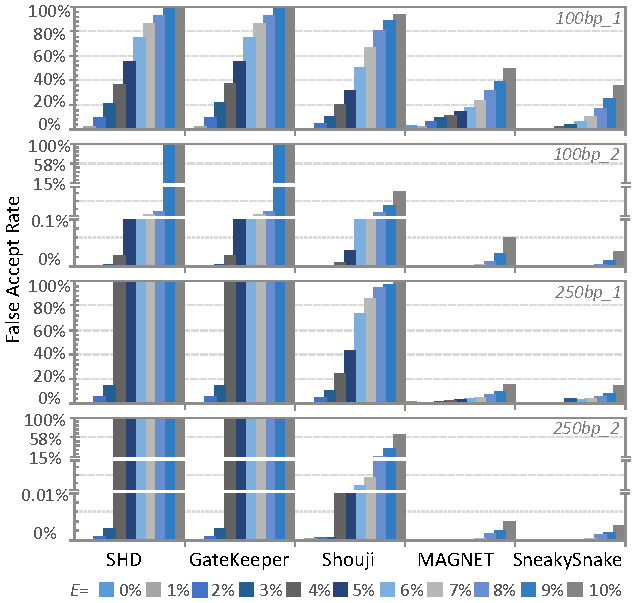
\includegraphics[width=1\linewidth]{figures/SS-fig5-false-accept-rate.pdf}}
\caption{{False accept rates of SHD, GateKeeper, Shouji, MAGNET, and SneakySnake across 4 real datasets of short sequences}. We use a wide range of edit distance thresholds ($0\%-10\%$ of the sequence length) for sequence lengths of 100 and 250 bp.}
\label{fig:false-accept-rate}
\end{figure}


\subsection{{Effect} of SneakySnake on Short Sequence Alignment}
We analyze the benefits of integrating CPU-based pre-alignment filters, SneakySnake and SHD with the state-of-the-art CPU-based sequence aligners, Edlib and Parasail. We evaluate all tools using a single CPU core and single thread environment. Fig. \ref{fig:CPUSneakySnake}(a) and (b) present the normalized end-to-end execution time of SneakySnake and SHD{,} each combined with Edlib and Parasail, using our four real datasets over edit distance thresholds of $0\%-10\%$ of the sequence length. We make four key observations. (1) The addition of SneakySnake as a pre-alignment filtering step {significantly} reduces the execution time of Edlib and Parasail by up to 37.7$\times$ (using \texttt{250bp\_2}, $E$= 0\%) and 43.9$\times$ (using \texttt{250bp\_2}, $E$ =2\%), respectively. 
We also observe a similar trend as the number of CPU threads increases from 1 to 40, as we {show} in Supplementary Materials, Section 10.2.
{To explore the reason for this significant speedup, we need to check how fast SneakySnake examines the sequence pairs compared to sequence alignment, which we observe next}.
(2) SneakySnake is up to 43$\times$ (using \texttt{250bp\_1}, $E$= 0\%) and  47.2$\times$ (using \texttt{250bp\_1}, $E$= 2\%) faster than Edlib and Parasail, respectively, in examining the sequence pairs. 
(3) SneakySnake provides up to 8.9$\times$ 
%(using Set\_4, $E$= 4\%) 
and 40$\times$ 
%(using Set\_4, $E$= 5\%) 
more speedup to the end-to-end execution time of Edlib and Parasail compared to SHD. This is expected as SHD produces a high false accept rate (as we show earlier in Section \ref{filtering_accuracy}).
(4) The addition of SHD as a pre-alignment step reduces the execution time of Edlib and Parasail for some of the edit distance thresholds by up to 17.2$\times$ (using \texttt{100bp\_2}, $E=0\%$) and 34.9$\times$ (using \texttt{250bp\_2}, $E$= 3\%), respectively. 
However, for most of the edit distance thresholds, we observe that Edlib and Parasail are faster alone than with SHD combined as a pre-alignment filtering step. This is expected as SHD becomes ineffective in filtering for $E$> 8\% and $E$> 3\% for $m$= 100 bp and $m$= 250 bp, respectively, (as we show earlier in Section \ref{filtering_accuracy}).

We conclude that SneakySnake is the best-performing CPU-based pre-alignment filter in terms of both speed and accuracy. Integrating SneakySnake with sequence alignment algorithms is always beneficial for short sequences and reduces the end-to-end execution time by up to an order of magnitude without the need for hardware accelerators. 
We also conclude that SneakySnake's performance {scales well} over a wide range of edit distance thresholds, number of CPU threads, and sequence lengths.


\begin{figure}
\centerline{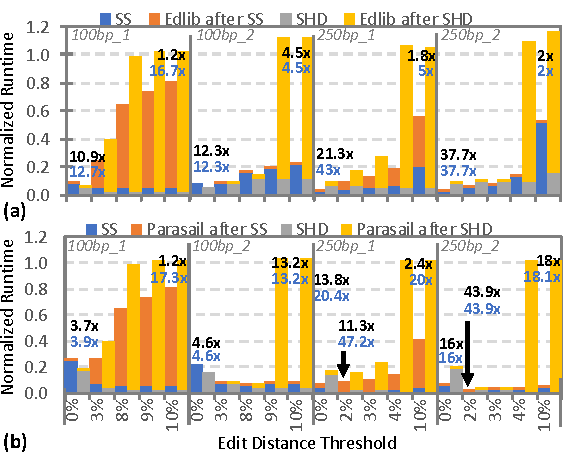
\includegraphics[width=1\columnwidth]{figures/Figure4-Oct2020.pdf}}
%\centerline{\includegraphics[width=0.8\textwidth]{figures/Figure4-March2020.pdf}}
\caption{\alser{Normalized end-to-end execution time of SneakySnake and SHD{, each} combined with (a) Edlib and (b) Parasail. 
{The execution time values in (a) and (b) are normalized to that of Edlib and Parasail, respectively, {without} pre-alignment filtering.}
We use four datasets over a wide range of edit distance thresholds ($E$= 0\%-10\% of the sequence length) for sequence lengths ($m$) of 100 bp {(\texttt{100bp\_1} and \texttt{100bp\_2})} and 250 bp {(\texttt{250bp\_1} and \texttt{250bp\_2})}.
We present two speedup {values} for $E$= 0\% and $E$= 10\% of {each dataset} and some other $E$ values highlighted by arrows. The {top} speedup {value} {(in black)} represents the end-to-end speedup that is gained from combining the pre-alignment filtering step with the alignment step. It is calculated as $A/(B+C)$, where $A$ is the execution time of the sequence aligner before adding SneakySnake {(not plotted in graphs)}, $B$ is the execution time of SneakySnake, and $C$ is the execution time of the sequence aligner after adding SneakySnake. The {bottom} speedup {value} {(in blue)} is calculated as $A/B$.% and it represents the speedup that is gained from using SneakySnake instead of the sequence alignment algorithm to examine all given sequence pairs.
}}
\label{fig:CPUSneakySnake}
\end{figure}

\subsection{{Effect} of Snake-on-Chip and Snake-on-GPU on Sequence Alignment}

We analyze the benefits of integrating Snake-on-Chip and Snake-on-GPU with the state-of-the-art sequence aligners, designed for different computing platforms in Fig. \ref{fig:Snake-on-Chip}.
{We} compare the effect of combining Snake-on-Chip and Snake-on-GPU with {an} existing sequence aligner {to} that of two state-of-the-art FPGA-based pre-alignment filters, Shouji and GateKeeper. 
We also select four state-of-the-art sequence aligners that are implemented for CPU (Edlib and Parasail), GPU (GSWABE), and FPGA (FPGASW). 
We use \texttt{100bp\_1} and \texttt{100bp\_2} in this {evaluation, as GSWABE, Shouji, and GateKeeper work for only short sequences}. GSWABE and FPGASW are not open-source and not available to us. Therefore, we scale {their} reported number of computed entries of the DP matrix {per} second (i.e., GCUPS) as follows: (number of sequence pairs in \texttt{100bp\_1} or \texttt{100bp\_2})/(GCUPS/$100^2$). 
We design the hardware architecture of Snake-on-Chip for a sub-maze's width of 8 VRTs ($t$=8) and 3 module instances ($y$=3) per each sub-maze. 
We select this design choice as it allows for low FPGA resource utilization while maintaining {a} low false accept rate{, based on our analysis of} different $y$ and $t$ values on the false accept rate of Snake-on-Chip {(these results} are reported in the {Supplementary Excel File} and on the SneakySnake GitHub page). 
%in \textcolor{red}{Supplementary Materials, Section 10.5}. 

Based on Fig. \ref{fig:Snake-on-Chip}, we make two key observations. (1) The execution time of Edlib and Parasail reduces by up to 321$\times$ (using \texttt{100bp\_2} and $E$ = 5\%) and 536$\times$ (using \texttt{100bp\_2} and $E$ = 5\%), respectively, after the addition of Snake-on-Chip as a pre-alignment filtering step and by up to 413$\times$ (using \texttt{100bp\_2} and $E$ = 5\%) and 689$\times$ (using \texttt{100bp\_2} and $E$ = 5\%), respectively, after the addition of Snake-on-GPU as a pre-alignment filtering step.
That is 40$\times$ (321/8) to 51$\times$ (689/13.39) more speedup {than} that provided by adding SneakySnake as a pre-alignment filter, using \texttt{100bp\_2} and $E$ = 5\%. 
It is also up to 2$\times$ more speedup compared to that provided by adding Shouji and GateKeeper as a pre-alignment filter, using \texttt{100bp\_1} and E=5\% for Snake-on-Chip and using \texttt{100bp\_2} and E=5\% for Snake-on-GPU. 
(2) 
%FPGAs and GPUs based sequence aligners follow a similar trend to that we observe in the CPU implementations.
Snake-on-GPU provides up to 27.7$\times$ (using \texttt{100bp\_2} and $E$ = 5\%) and 5.1$\times$ (using \texttt{100bp\_2} and $E$ = 5\%) reduction in the end-to-end execution time of GSWABE and FPGASW, respectively. 
This is up to 1.3$\times$ more speedup {than} that provided by Snake-on-Chip, using \texttt{100bp\_2}. That is also up to 1.7$\times$ more speedup {than} that provided by adding Shouji and GateKeeper as a pre-alignment filter. 
{The speedup provided by Snake-on-GPU and Snake-on-Chip to GSWABE and FPGASW is less than that observed in Edlib and Parasail. This is due to the low execution time of hardware accelerated aligners.}

We conclude that both Snake-on-Chip and Snake-on-GPU provide the highest speedup (up to two orders of magnitude) {when combined with} the state-of-the-art CPU, FPGA, and GPU based sequence aligners over edit distance thresholds of 0\%-5\% of the sequence length.

\begin{figure}
\centerline{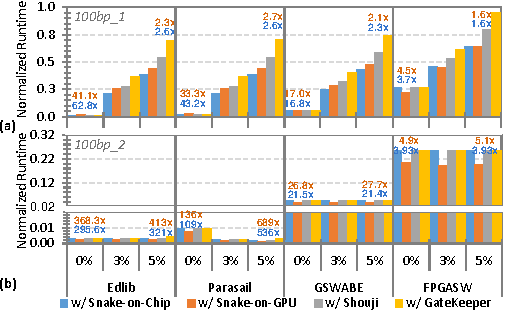
\includegraphics[width=1\linewidth]{figures/Figure5-Oct2020.pdf}}
\caption{\alser{Normalized end-to-end execution time of a pre-alignment filter (Snake-on-Chip, Snake-on-GPU, Shouji, and GateKeeper) combined with a sequence aligner (Edlib, Parasail, GSWABE, and FPGASW). {Each execution time value is normalized to that of the corresponding sequence aligner {without} pre-alignment filtering.}
We use two datasets, (a) \texttt{100bp\_1} and (b) \texttt{100bp\_2}, over a wide range of edit distance thresholds (0\%-10\% of the sequence length, 100 bp). We present two end-to-end speedup {values} for edit distance thresholds of 0\% and 5\%. The {top} speedup {value} {(in orange)} is the speedup gained from integrating Snake-on-GPU with the corresponding sequence aligner. The {bottom} speedup {value} {(in blue)} represents the speedup gained from integrating Snake-on-Chip with the corresponding sequence aligner.}}
\label{fig:Snake-on-Chip}
\end{figure}




%We now examine the execution time of SneakySnake, Parasail, and SneakySnake integrated with Parasail using long reads, as we show in Fig. 10. We run both SneakySnake and Parasail using two sets (Set\_5 and Set\_6) of long reads and 40 CPU threads. We run SneakySnake with $t$ = $y$ = (E+500), where $t$ is the width of the chip maze of each subproblem, $y$ is the number of iterations performed to solve each subproblem, and $E$ is the edit distance threshold. We choose the values of $t$ and $y$ to be less than the sequence length to prevent SneakySnake from examining the entire chip maze, which helps to achieve fast filtering at the cost of a slight increase in the number of falsely-accepted pairs (with a 0\% false reject rate). We also choose the values of $t$ and $y$ to be more than E to prevent the chip maze to have complete rows of obstacles based on Equation 1 in the main paper. 
%We experimentally evaluate the effect of varying the values of $t$ and $y$ on both the accuracy and execution time of short sequence filtering and alignment in \url{https://github.com/CMU-SAFARI/SneakySnake/tree/master/Evaluation\%20Results}. 
%We use a wide range of edit distance thresholds, up to 20\% of the sequence length. 

%Based on Fig. 10, we make two key observations. (1) Using Set\_5 and Set\_6, SneakySnake makes Parasail significantly faster (by 58.2-708.4$\times$ and by 50.9-978.8$\times$, respectively) than Parasail alone in detecting dissimilar pairs of long sequences, even at high edit distance thresholds (up to $E$=501 for Set\_5 and up to $E$=5010 for Set\_6, which result in building and examining 1003 and 10021 rows, respectively, for each chip maze of the SneakySnake algorithm). (2) As the number of similar sequence pairs increases (at E > 501 for Set\_5 and at E > 5010 for Set\_6), the benefits of integrating SneakySnake with Parasail in reducing the end-to-end execution time becomes less. As 89\% and 94\% of the input sequence pairs passed SneakySnake to Parasail using Set\_5 and Set\_6, respectively, integrating SneakySnake with Parasail shows almost the same end-to-end execution time of Parasail alone. This is expected, as each sequence pair that passed SneakySnake is examined unnecessarily twice (i.e., once by SneakySnake and once by Parasail). 
%We provide the exact values of all evaluation results in \url{https://github.com/CMU-SAFARI/SneakySnake/tree/master/Evaluation\%20Results}.

\subsection{{Effect} of SneakySnake on Long Sequence Alignment}
{We} examine the benefits of integrating SneakySnake with Parasail~\citep{daily2016parasail} and KSW2~\citep{suzuki2018introducing, li2018minimap2} {for long sequence alignment} (\texttt{100Kbp}). 
We run Parasail as nw\_banded. We run KSW2 as extz2\_sse, a global alignment implementation that is parallelized using the Intel SSE instructions{. KSW2} uses heuristics~\citep{suzuki2018introducing} to improve the alignment time. We run SneakySnake with Parasail using 40 CPU threads. We run SneakySnake with KSW2 using a single CPU thread (as KSW2 does not support multithreading). We use a wide range of edit distance thresholds, up to 20\% of the sequence length.

Based on Table \ref{table:1}, we make two key observations. (1) SneakySnake {accelerates} Parasail and KSW2 by 50.9-979$\times$ and 3.8-91.7$\times$, respectively, even at high edit distance thresholds (up to $E$=5010 (5\%), which results in building and examining a chip maze of 10,021 rows for each sequence pair).
(2) As the number of similar sequence pairs increases, the {performance benefit} of integrating SneakySnake with Parasail and KSW2 in reducing the end-to-end execution time {reduces}. 
{When Parasail and KSW2 examine 94\% and 73\% of the input sequence pairs (SneakySnake filters out the rest of the sequence pairs), respectively, SneakySnake provides slight or no performance benefit to the end-to-end execution time of the sequence aligner alone}. 
This is expected, as each sequence pair that passes SneakySnake is examined unnecessarily twice (i.e., once by SneakySnake and once by sequence aligner). We provide more details on this evaluation for both \texttt{10Kbp} and \texttt{100Kbp} in Supplementary Materials, Section 10.3.
We observe that SneakySnake accelerates Parasail and KSW2 by 276.9$\times$ and 31.7$\times$ on average, respectively, when {sequence alignment examines at most 73\% of the input sequence pairs}.

We conclude that {when SneakySnake filters out more than 27\% of the input sequence pairs, integrating SneakySnake with long sequence aligners is always beneficial and sometimes reduces the end-to-end execution time by one to two orders of magnitude (depending on the edit distance threshold and how fast the sequence aligner examines the input sequence pairs compared to SneakySnake) without the need for hardware accelerators}.


\begin{table}[H]
\caption{The end-to-end execution time (in seconds) of SneakySnake integrated with Parasail (40 CPU threads) and KSW2 (single threaded) using long reads (\texttt{100Kbp}).}
\label{table:1}
\centering
\begin{tabularx}{\linewidth}{c|rrrrr}
\hline
\textit{\textbf{E}} & \multicolumn{1}{l}{\textbf{Parasail}} & \multicolumn{1}{l}{\textbf{SS+Parasail}} & \multicolumn{1}{l}{\textbf{KSW2}} & \multicolumn{1}{l}{\textbf{SS+KSW2}} &  
\begin{minipage}[c] [.7cm] [c] {0.15\columnwidth}%
\centering
\textbf{SS Accept Rate} %
\end{minipage}
\\ \hline
0.01\% & 84.0 & \textbf{0.23} & 1380.2 & \textbf{15.1} & 0\% \\
0.3\% & 2,756.3 & \textbf{2.8} & 8,215.5 & \textbf{135.4} & 0\% \\
5.0\% & 37,492.3 & \textbf{736.5} & 100,178.3 & \textbf{26,261.4} & 0\% \\
10.7\% & 81,881.6 & \textbf{49,322.1} & 204,135.3 & \textbf{184,312.5} & 57\% \\
10.8\% & 82,646.1 & \textbf{63,756.0} & 206,041.4 & 225,815.2 & 73\% \\
11.0\% & 84,098.7 & \textbf{83,437.5} & 209,662.8 & 287,206.8 & 94\% \\
12.0\% & 91,744.1 & 95,533.6 & 228,723.1 & 325,966.0 & 100\% \\
20.0\% & 152,906.8 & 157,982.0 & 381,205.1 & 544,282.1 & 100\% \\ \hline
\end{tabularx}
\end{table}


%\begin{table}[H]
%\caption{The end-to-end execution time (in seconds) of SneakySnake integrated with Parasail (40 CPU threads) and KSW2 (single threaded) using long reads (\texttt{100Kbp}).}
%\label{table:1}
%\centering
%\begin{tabularx}{\linewidth}{c|rrrrr}
%ine
%\textit{\textbf{E}} & \multicolumn{1}{l}{\textbf{Parasail}} & \multicolumn{1}{l}{\textbf{SS+Parasail}} & \multicolumn{1}{l}{\textbf{KSW2}} & \multicolumn{1}{l}{\textbf{SS+KSW2}} &  
%\begin{minipage}[c] [.7cm] [c] {0.15\columnwidth}%
%\centering
%\textbf{SS Accept Rate} %
%\end{minipage}
%\\ ine
%0.01\% & 84.0 & \textbf{0.23} \small{(351.5$\times$)} & 1380.2 & \textbf{15.1} \small{(91.7$\times$)} & 0\% \\
%0.3\% & 2,756.3 & \textbf{2.8} \small{(979$\times$)} & 8,215.5 & \textbf{135.4} \small{(60.6$\times$)} & 0\% \\
%5.0\% & 37,492.3 & \textbf{736.5} \small{(50.9$\times$)} & 100,178.3 & \textbf{26,261.4} \small{(3.8$\times$)} & 0\% \\
%10.7\% & 81,881.6 & \textbf{49,322.1} \small{(1.7$\times$)} & 204,135.3 & \textbf{184,312.5} \small{(1.1$\times$)} & 57\% \\
%10.8\% & 82,646.1 & \textbf{63,756.0} \small{(1.3$\times$)} & 206,041.4 & 225,815.2 \small{(0.91$\times$)} & 73\% \\
%11.0\% & 84,098.7 & \textbf{83,437.5} \small{(1$\times$)} & 209,662.8 & 287,206.8 \small{(0.73$\times$)} & 94\% \\
%12.0\% & 91,744.1 & 95,533.6 \small{(0.96$\times$)} & 228,723.1 & 325,966.0 \small{(0.7$\times$)} & 100\% \\
%20.0\% & 152,906.8 & 157,982.0 \small{(0.97$\times$)} & 381,205.1 & 544,282.1 \small{(0.7$\times$)} & 100\% \\ ine
%\end{tabularx}
%\end{table}


\subsection{{Effect} of SneakySnake on Read Mapping}
\alser{After confirming the benefits of the different implementations of the SneakySnake algorithm, {we} evaluate the overall benefits of integrating SneakySnake with minimap2 (2.17-r974-dirty, 22 January 2020) \citep{li2018minimap2}. 
We select minimap2 for two main reasons. (1) It is a state-of-the-art read mapper that includes efficient methods (i.e., minimizers and seed chaining) for accelerating read mapping. (2) It utilizes a banded global sequence alignment algorithm (KSW2, implemented as \emph{extz2\_sse}) that is parallelized and accelerated using both the Intel SSE instructions and heuristics \citep{suzuki2018introducing} to improve the alignment time.
We map all reads from ERR240727\_1 (100 bp) to GRCh37 with edit distance thresholds of 0\% and 5\% of the sequence length. 
{We run minimap2 using --sr mode (short read mapping) and the default parameter values.}
We replace the seed chaining %(lines 305 to 358 of \emph{map.c} file) 
of minimap2 with SneakySnake.
In these experiments, we ensure that we maintain the \emph{same} reported mappings for both tools. 
We make two observations. 
(1) SneakySnake and the minimap2's aligner (KSW2) together are at least 6.83$\times$ (from 246 seconds to 36 seconds) and 2.51$\times$ (from 338 seconds to 134.67 seconds) faster than the minimap2's seed chaining and the minimap2's aligner together for edit distance thresholds of 0\% and 5\%, respectively. 
(2) The mapping time of minimap2 reduces by a factor of up to 2.01$\times$ (from 418 seconds to 208 seconds) and 1.66$\times$ (from 510 seconds to 306.67 seconds) after integrating SneakySnake with minimap2 for edit distance thresholds of 0\% and 5\%, respectively.}

{We conclude that SneakySnake is {very} beneficial even for minimap2, a state-of-the-art read mapper, which uses minimizers, seed chaining, and SIMD-accelerated banded alignment.
This promising result motivates us to explore in detail accelerating minimap2 using Snake-on-GPU and Snake-on-Chip in our future research.}
%After confirming the benefits of integrating SneakySnake and Snake-on-Chip with sequence aligners, we now evaluate the overall benefits of integrating SneakySnake and Snake-on-Chip with the mrFAST (version 2.6.1) read mapper \citep{alkan2009personalized}. We select mrFAST for two main reasons. (1) It already includes the Adjacency Filter \citep{xin2013accelerating} as a pre-alignment step, so it constitutes a state-of-the-art baseline. (2) It utilizes a banded Levenshtein edit distance algorithm \citep{ukkonen1985algorithms} that is parallelized using the Intel SSE instructions, and thus it utilizes the capabilities of state-of-the-art hardware. Fig. \ref{fig:mrFAST} presents the effect of SneakySnake and Snake-on-Chip on the overall mapping time, when all reads from ERR240727\_1 (100 bp) are mapped to GRCh37 with edit distance thresholds of 0\% to 5\%. We make two observations. (1) SneakySnake and Snake-on-Chip are at least 10.8$\times$ and 675.1$\times$ faster than mrFAST's banded Levenshtein edit distance algorithm. (2) The verification time of mrFAST reduces by a factor of up to 2.93$\times$ and 7.57$\times$ after replacing the Adjacency Filter with SneakySnake and Snake-on-Chip, respectively, as the pre-alignment filtering step.

%\begin{figure}
%\centerline{\includegraphics[width=0.8\linewidth]{figures/SneakySnake-mrFast.pdf}}
%\caption{Normalized end-to-end execution time of mrFAST (version 2.6.1) mapper combined with SneakySnake and Snake-on-Chip. We use mrFAST to map all reads from ERR240727\_1 (100 bp) to the human reference genome, GRCh37, over edit distance thresholds of 0\%-5\% of the sequence length, 100 bp. We present the end-to-end speedup rates that SneakySnake and Snake-on-Chip provide for mrFAST.}
%\label{fig:mrFAST}
%\end{figure}
